\begin{figure}[htbp]
  \centering
  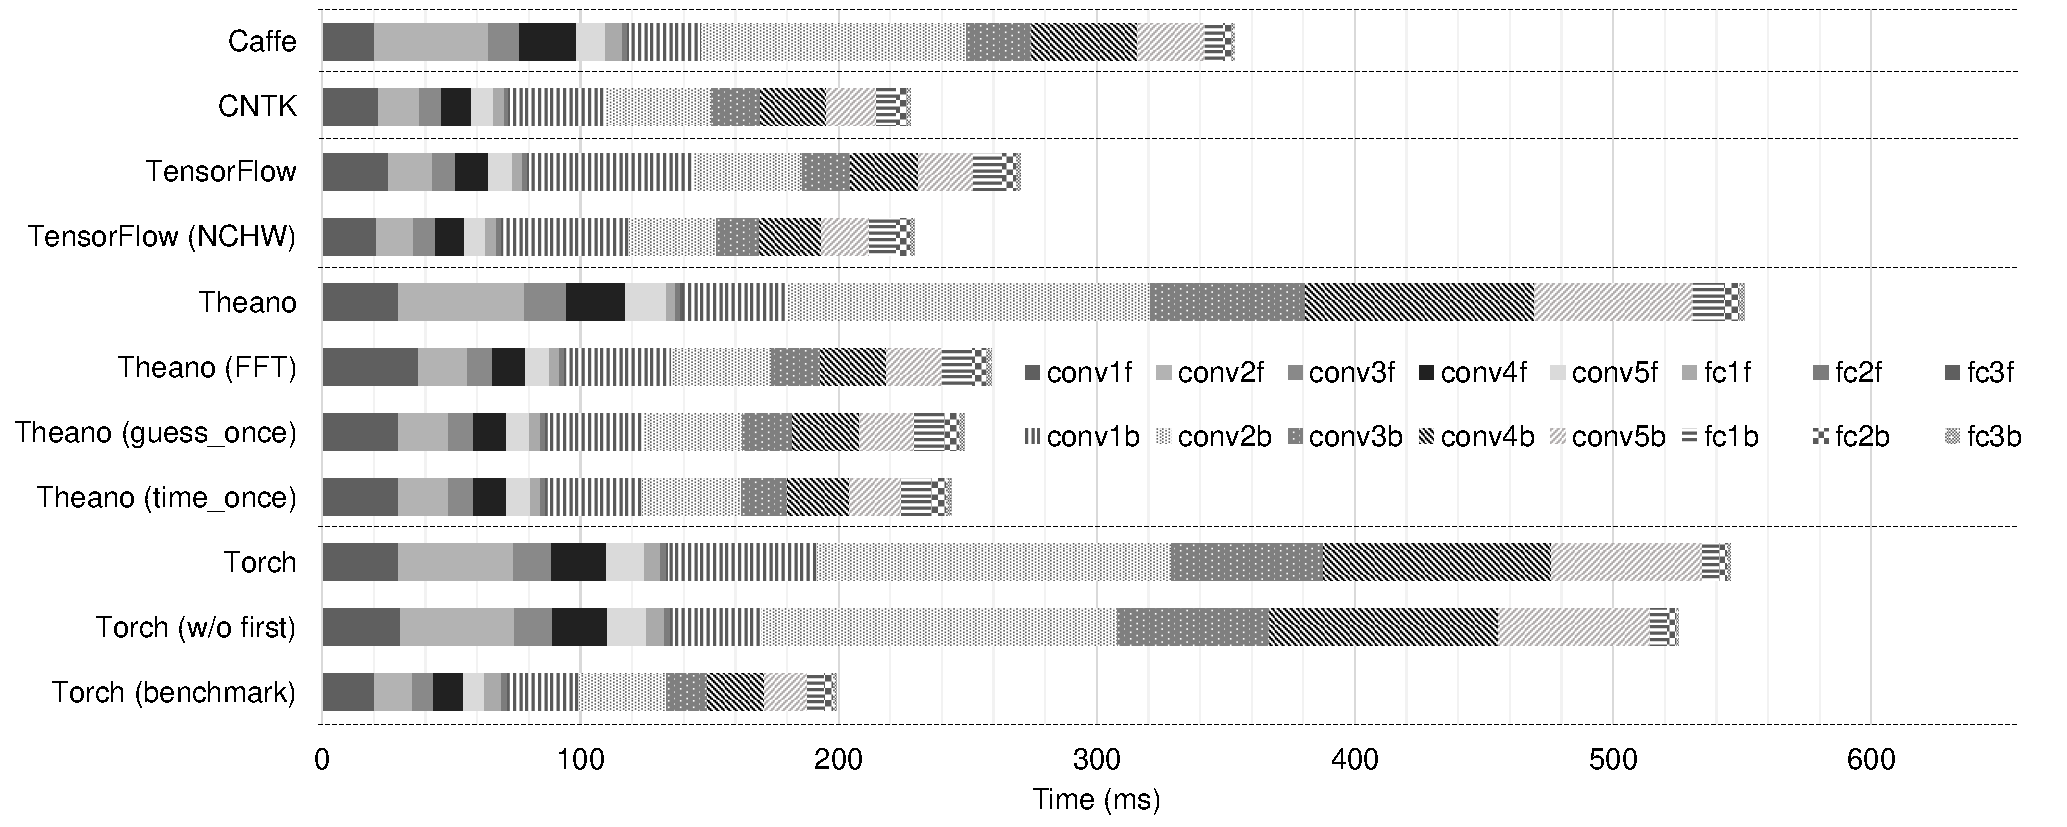
\includegraphics[width=\linewidth]{./figures/time_frameworks}
  \caption{%
The execution time of training AlexNet with a batch of imput images for differnt deep learning frameworks. 
\label{fig_time_frameworks}
  }
\end{figure}

%A = Caffe, B = TensorFlow, C = TensorFlow (NCHW tensor), D = Theano, E = Theano (FFT), F = Theano (guess\_once), G = Theano (time\_once), H = Torch, I = Torch (no backward propagation in the first layer), J = Torch (FFT), K = Torch (benchmarking) 

\section{Charactrization on a Single GPU}
\label{sec:singlGPU}
In this section, we characterize the five deep learning frameworks on a single GPU. The measurement of the layer-wise execution time of the AlexNet model for each framework is shown in Figure~\ref{fig_time_frameworks}. We observe that slight changes in framework options result in large performance differences. Options for convolution algorithm choices, data layout, and disabling useless backpropagation are most influential. We can increase the speed of training a CNN model up to 2X by just changing framework options. We do not need to modify the source code of the framework at all. 

%그 외 사소한 것으로 텐서에 네트워크 입력을 feed_dict로 주면 CPU 복사가 일어나서 매우 느리므로 FixedLengthRecordReader 등으로 주는게 좋다.
%https://github.com/tensorflow/tensorflow/issues/2919

%https://github.com/BVLC/caffe/blob/rc3/src/caffe/layers/cudnn_conv_layer.cpp#L113
%https://github.com/tensorflow/tensorflow/blob/v0.10.0rc0/tensorflow/core/kernels/conv_ops.cc#L460
%https://github.com/tensorflow/tensorflow/blob/v0.10.0rc0/tensorflow/stream_executor/cuda/cuda_dnn.cc#L933
%https://github.com/Theano/Theano/blob/rel-0.8.2/theano/sandbox/cuda/dnn.py#L285
%https://github.com/Theano/Theano/blob/rel-0.8.2/theano/sandbox/cuda/dnn_fwd.c#L227
%https://github.com/soumith/cudnn.torch/blob/R5/SpatialConvolution.lua#L166

